% Ubah judul dan label berikut sesuai dengan yang diinginkan.
\section{Desain dan Implementasi Sistem}
\label{sec:desainimplementasi}

Paper ini membahas mengenai implementasi salah satu cabang ilmu dalam \textit{deep learning}, yang bertujuan untuk mendeteksi suatu berita hoaks berbahasa indonesia secara otomatis menggunakan metode BERT. Pendeteksi ini dilatih menggunakan gabungan dataset dari \url{https://data.mendeley.com/datasets/p3hfgr5j3m/1} dan dataset yang kami buat sendiri menggunakan teknologi \textit{web crawling}. Gambar \ref{fig:metodologi} merupakan garis besar penelitian ini.

\begin{figure} [ht]
    \centering
    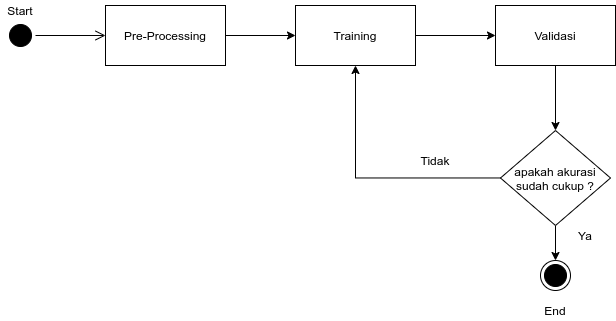
\includegraphics[width=0.4\textwidth]{gambar/Metodologi.png}
    \caption{Garis besar metodologi penelitian.}
    \label{fig:metodologi}
\end{figure}

\subsection{Material dan Spesifikasi Alat}

Pada penelitian ini, dataset yang digunakan adalah dataset yang berasal dari \url{https://data.mendeley.com/datasets/p3hfgr5j3m/1} yang digabungkan dengan dataset yang kami buat sendiri menggunakan teknologi \textit{web crawling}. Total dataset yang berhasil kami kumpulkan adalah 1621 data dengan rincian tertera pada tabel \ref{tab:dataset}, sedangkan pada tabel \ref{tab:dataset_mendeley} merupakan dataset awal yang kami dapatkan dari \url{data.mendeley.com}.

Dataset tersebut berisi isi berita disertai dengan label Valid atau Hoaks. Sumber berita dataset yang kami gunakan berasal dari berbagai sumber yang sudah terakreditasi untuk berita yang valid, dan dari berbagai sumber yang kurang terakreditasi untuk berita yang hoaks. Tabel \ref{tab:contoh_dataset} merupakan contoh sebagian data yang kami gunakan dalam penelitian ini.

\begin{table}
    \caption{Jumlah Dataset dari \url{data.mendeley.com}}
    \label{tab:dataset_mendeley}
    \centering
    \begin{tabular}{ | l | l | }
        \hline
        \textbf{Label} & \textbf{Jumlah Data} \\ \hline
        \textit{Hoaks} & 228                  \\ \hline
        \textit{Valid} & 372                  \\ \hline
        \textbf{Total} & \textbf{600}         \\ \hline
    \end{tabular}
\end{table}

\begin{table}
    \caption{Jumlah Dataset yang digunakan}
    \label{tab:dataset}
    \centering
    \begin{tabular}{ | l | l | }
        \hline
        \textbf{Label} & \textbf{Jumlah Data} \\ \hline
        \textit{Hoaks} & 885                  \\ \hline
        \textit{Valid} & 736                  \\ \hline
        \textbf{Total} & \textbf{1621}        \\ \hline
    \end{tabular}
\end{table}


\begin{table}
    \caption{Contoh Dataset}
    \label{tab:contoh_dataset}
    \centering
    \begin{tabular}{ | p{.8\linewidth} | l | }
        \hline
        \textbf{berita}                                                                                                                                                                                                                   & \textbf{\textit{tagging}} \\ \hline
        Wakil Gubernur DKI Jakarta Sandiaga Uno menargetkan pengerjaan tahap awal Stadion BMW dilakukan pada Oktober. Stadion ini diperuntukkan bagi klub Persija....                                                                     & Valid                     \\ \hline
        "Komisi II bersama KPU dan Bawaslu masih membahas ketentuan wajib cuti bagi petahana presiden yang maju Pilpres 2019. Mekanisme pengambilan.....                                                                                  & Valid                     \\ \hline
        Jaksa penuntut Ulumum (JPU) pada Komisi Pemberantasan Korupsi (KPK) mencecar Pejabat Pembuat Komitmen (PPK) reguler pada Direktorat Perlindungan Sosial Korban Bencana Sosial Kemensos Victorious Saut Hamonangan Siahaan soal... & Valid                     \\ \hline
        “Halo Kak! Aku Winda Dari Team Giveaway BAIM WONG Anda Memenangkan Hadiah Uang 100Jt dari kami info klik: https://wa.me/+6285796306857”                                                                                           & Hoax                      \\ \hline
        “Apa yang terjadi dengan hewan dalam penelitian?   Teknologi ini telah dicoba pada hewan, dan pada hewan penelitian yang dilakukan, semua hewan mati , tidak langsung dari suntikan...                                            & Hoax                      \\ \hline
        “Kadrun istilah dr PKI alias KOMUNIS ditujukan buat islam. Kl mau jd komunis pake aja istilah kadrun buat umat islam. Auto lsg Komunis”                                                                                           & Hoax                      \\ \hline
    \end{tabular}
\end{table}

\subsection{Pembuatan Dataset}
Berhubung dataset dari \url{https://data.mendeley.com/datasets/p3hfgr5j3m/1} dirasa sangat kurang karena hanya berjumlah 600 data saja. Maka dari itu kami membuat sebuah program \textit{web crawling} yang digunakan untuk mengambil teks berita dari beberapa situs berita yang sudah terakreditasi seperti \url{liputan6.com}, \url{detik.com}, \url{tempo.com}. Sedangkan untuk teks berita hoaks, sumber yang kami gunakan adalah \url{turnbackhoax.id}.

Gambar \ref{fig:webcrawl_method} adalah gambaran garis besar yang kami lakukan dalam program \textit{web crawl} kami. Dimulai dengan memasukkan kode HTML mentah, kemudian merubah kode mentah tersebut menjadi objek yang lebih mudah untuk dilakukan pemrosesan dalam python, mengambil teks berita dan melakukan pembersihan terhadap teks tersebut, terakhir menghasilkan keluaran berupa file .CSV dengan format yang sesuai.

\begin{figure} [ht]
    \centering
    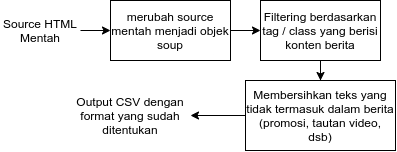
\includegraphics[width=0.4\textwidth]{gambar/webcrawl.png}
    \caption{Garis besar alur program \textit{web crawl}.}
    \label{fig:webcrawl_method}
\end{figure}

\begin{lstlisting}[
  language=Python,
  caption={Program \textit{web crawling} \url{detik.com}.},
  label={lst:webcrawl_detik}
]
source = soup.find(class_="detail__body-text")

        result_text = ""

        for text in source.find_all("p"):

            # skpping on editorial notes and video promote
            if (text.find("strong")):
                continue

            # skipping video promote
            if(text.find("a", class_='embed')):
                continue

            result_text = result_text + text.get_text()
\end{lstlisting}

\textit{Library} yang kami gunakan untuk melakukan \textit{crawling} adalah \textit{BeautifulSoup}, sebuah \textit{library} yang akan secara otomatis merubah dari suatu teks HTML menjadi objek \textit{soup} yang lebih mudah untuk dilakukan pemrosesan di dalam python. Listing \ref{lst:webcrawl_detik} adalah salah satu bagian dari \textit{web crawling} yang kami gunakan untuk mengambil teks berita dari situs \url{detik.com}

\begin{lstlisting}[
    language=HTML, 
    caption={Penggalan Kode Sumber HTML \url{detik.com}.},
    label={lst:source_detik}
]

...
<div class="detail__body itp_bodycontent_wrapper">
<div class="detail__body-text itp_bodycontent">

<strong>Jakarta</strong> - Koalisi <a href="https://
detik.com/tag/jokowi" target="_blank">Jokowi</a> 
sedang menyusun visi-misi jagoannya. Setelah 
menerima masukan dari <a href="https://detik.com/
tag/muhammadiyah" target="_blank"> Muhammadiyah</a>,
 ... 
Dan kita pun membuka diri untuk menerima 
masukan untuk penyempurnaan," imbuhnya.<br><br><!--
s:parallaxindetail--><div class="clearfix"></div><style>
...

\end{lstlisting}

Yang pertama kali harus kami lakukan adalah menentukan \textit{tag} atau \textit{class} HTML yang akan kami gunakan untuk melakukan penyaringan terlebih dahulu. Apabila merujuk pada listing \ref{lst:source_detik} \textit{class} yang berisi teks seluruh berita adalah \texttt{detail\_\_body\-text} sehingga kami melakukan penyaringan dengan memasukkan \textit{class} tersebut ke dalam parameter dengan cara \texttt{ source = soup.find(class\_="detail\_\_body\-text") }.

Namun, walaupun sudah melakukan penyaringan, masih terdapat beberapa teks yang tidak diperlukan seperti catatan dari penulis, dan tautan untuk menuju ke berita yang masih berhubungan. Sehingga, setelah melakukan penyaringan, masih diperlukan lagi pembersihan isi berita dari teks - teks yang tidak diperlukan.

\begin{lstlisting}[
  language=Python,
  caption={Program keluaran \textit{web crawl} \url{detik.com}.},
  label={lst:output_webcrawl}
]
with open(result_files, "w", newline="") as file:
    mywriter = csv.writer(file, delimiter=",")
    mywriter.writerow(["url", "judul", "berita", "tagging"])

    for data in listNews:
        mywriter.writerow(
            [data.url, data.title, data.content, 
            self.validString(data.valid)])

\end{lstlisting}

Terakhir, adalah melakukan keluaran berupa \textit{file} .CSV. Listing \ref{lst:output_webcrawl} adalah penggalan program untuk menghasilkan keluaran dengan tipe data CSV.

\subsection{Preprocessing}

\begin{figure}[h!]
    \begin{center}
        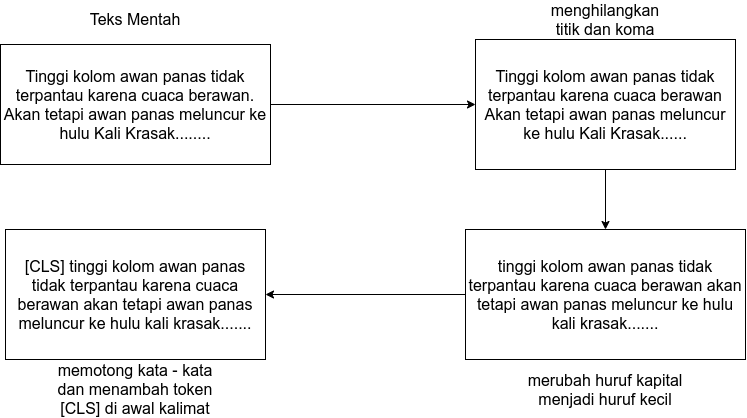
\includegraphics[width= 0.8\linewidth]{gambar/preprocess.png}
        \caption{Metode Preprocessing}
        \label{fig: metodologi_preprocessing}
    \end{center}
\end{figure}

Pada proses ini, data akan disiapkan terlebih dahulu agar dapat diproses oleh BERT. Proses penyiapan data meliputi menghilangkan titik dan koma, dan merubah huruf kapital yang ada menjadi huruf kecil seluruhnya. Dan karena BERT memiliki maksimal kata - kata yang dapat diproses dalam sekali waktu sejumlah 512 kata atau token, maka harus dilakukan penyingkatan teks, dapat dengan cara melakukan pengambilan 512 karakter pertama, terakhir maupun gabungan dari kedua bentuk. Langkah terakhir adalah menambahkan token \texttt{[CLS]} di awal kalimat. Untuk lebih jelasnya, bisa melihat pada Gambar \ref{fig: metodologi_preprocessing}.

Selain itu, juga akan dilakukan pembagian dataset yang awalnya berjumlah 1621 akan dibagi menjadi 3 bagian dengan ketentuan :

\begin{itemize}
    \item 70\% \textit{Training}, 10\% Validasi, 20\% Pengujian
\end{itemize}

\begin{enumerate}
    \item \textit{Training}

          Set ini digunakan oleh algoritma BERT sebagai masukan saat melakukan proses \textit{training} sehingga akan didapat model yang sesuai.

    \item Validasi

          Set ini digunakan pada saat selesai melakukan validasi model setelah melakukan \textit{training}. Digunakan untuk menentukan apakah suatu model sudah memiliki \textit{weight} yang sesuai ataukah masih perlu melakukan \textit{training} lagi. Selain itu, set ini juga digunakan untuk menghindari kemungkinan \textit{overfitting} maupun \textit{underfitting} dalam model.

    \item Pengujian

          Set yang digunakan untuk melakukan pengujian akurasi model setelah proses \textit{training} dan validasi selesai. Hasil akurasi dari pengujian inilah yang akan digunakan sebagai hasil dari model.

\end{enumerate}

\subsection{Training}

\begin{figure}[h!]
    \begin{center}
        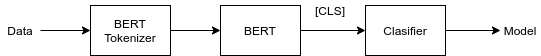
\includegraphics[width= 0.9\linewidth]{gambar/training.png}
        \caption{Metode Training}
        \label{fig: metodologi_training}
    \end{center}
\end{figure}

Pada tahap ini, teks yang sudah melewati proses \textit{preprocessing} akan dilakukan proses Tokenizer. Tokenizer adalah proses untuk merubah kata - kata dalam teks menjadi token sesuai dengan \textit{word embedding} yang sudah ada pada \textit{pretrained} BERT. Barulah pada saat itu, BERT dapat melakukan \textit{training} berdasarkan data dari \textit{dataset}.

Keluaran dari BERT akan diambil isi token \texttt{[CLS]}-nya dan dimasukkan kedalam algoritma klasifikasi, seperti \textit{Linear Regression}. \textit{Linear Regression} digunakan sebagai algoritma klasifikasi yang cukup mudah namun memiliki tingkat akurasi yang cukup. Gambar \ref{fig: metodologi_training} dapat digunakan sebagai penjelas.

Pada tahap ini juga dilakukan pengaturan ukuran \textit{batch}, \textit{learning rate} dan juga \textit{epoch}. \textit{Batch} adalah banyaknya teks yang diproses untuk setiap iterasi, semakin tinggi nilai \textit{batch} yang dikonfigurasi, maka proses \textit{training} akan semakin cepat namun memakan memori yang lebih banyak. Berhubung algoritma BERT adalah algoritma yang cukup berat karena memiliki \textit{layer} yang cukup banyak, maka dalam penelitian ini kami menggunakan \textit{batch} dengan nilai 8.

\textit{Epoch} adalah berapa banyak suatu algoritma melakukan proses \textit{training} dan validasi sebelum dianggap final. Disini \textit{epoch} harus diperhatikan agar jumlah \textit{loss} yang terjadi pada saat proses \textit{training} tidak terlalu tinggi karena merupakan ciri - ciri \textit{underfitting} namun juga tidak terlalu rendah selama beberapa \textit{epoch} untuk menghindari kemungkinan \textit{overfitting}. Berhubung kami hanya menggunakan BERT untuk memproses teks yang relatif lebih mudah, kami hanya menggunakan \textit{epoch} sebesar 10.

\textit{learning rate} adalah seberapa banyak \textit{hiperparameter} yang dirubah selama proses \textit{training}. \textit{hiperparameter} digunakan untuk merubah \textit{weight} selama proses \textit{training} berdasarkan \textit{feedback} saat proses validasi. Disini kami menggunakan nilai yang direkomendasikan oleh pembuat model BERT yang kami gunakan, yaitu 0.00002 \cite{koto2020indolem}.

\subsection{Validasi}

Dari model yang sudah dibentuk pada saat proses \textit{training}, akan dilakukan pengujian terhadap data yang sama sekali baru dan tidak digunakan selama proses \textit{trainig}. Hal ini untuk menghindari bias yang mungkin terjadi apabila model diuji pada data yang sama yang digunakan pada saat proses \textit{training}. Proses inilah yang disebut dengan proses validasi.

Berdasarkan dari data akurasi yang didapat dari proses validasi, maka dapat diambil keputusan apakah masih diperlukan optimisasi dan melakukan \textit{training} lagi, atau akurasi yang didapat sudah dianggap cukup baik.

\subsection{Pengujian}

Setelah melakukan proses validasi dan \textit{training}, maka yang harus dilakukan adalah melakukan pengujian terhadap model yang sudah dibuat. Dari proses ini dapat diambil kesimpulan apakah model tersebut sudah cukup baik, ataukah masih dapat dilakukan perbaikan atau optimisasi lagi salah satunya dengan cara mengatur ulang konfigurasi - konfigurasi yang sudah diatur pada saat proses \textit{training}.
